% The model
%-----------------------------------------------------------------------------
%   - Introduction
%   - Why iso and gyro are independent
%   - The formulas
%   - A description and reiteration in words.

% PGM
%-----------------------------------------------------------------------------
%   - The PGM
%   - A description of the PGM

% Practicalities: sampling, etc.
%-----------------------------------------------------------------------------
%   - Emcee
%   - Assessing convergence


% The model
%-----------------------------------------------------------------------------

%   - Introduction
In Bayesian statistics, combining information from different models can be
relatively simple, as long as the processes being modeled, that generated the
data, are independent.
In this case, we are combining information that relates to the burning of
hydrogen in the core (this is the process that drives the slow increase in
\teff\ and luminosity over time) with information about the magnetic braking
history of a star (rotation period).
We can assume that, to first order, these two processes are independent: the
hydrogen fraction in the core does not affect a star's rotation period and
vice versa.
In practise we can never be entirely sure that two such processes are
independent but, at least within the uncertainties, any dependence here is
unlikely to affect our results.
If this assumption is valid, then the likelihoods calculated using each model
can be multiplied together.

The desired end product of this method is an estimate of the non-normalized
posterior probability density function (PDF) over the age of a star,
\begin{equation}
p(A|{\bf m_x}, T_{\mathrm{eff}}, \log g, \hat{F}, P_{rot}, \bar{\omega}),
\end{equation}
where $A$ is age, ${\bf m_x}$ is a vector of apparent magnitudes in various
bandpasses (in our model ${\bf m_x} = [m_J, m_H, m_K]$), $\hat{F}$ is the {\it
observed} bulk metallicity, $P_{\mathrm{rot}}$ is the rotation period and
$\bar{\omega}$ is parallax.
In order to calculate a posterior PDF over age, we must marginalize over
parameters that relate to age, but are not of interest in this study: mass
($M$), distance ($D$), V-band extinction ($A_V$) and an {\it inferred} bulk
metallicity, $\mathrm{F}$.
The marginalization involves integrating over these extra parameters,
\begin{eqnarray}
& p(A|{\bf m_x}, T_{\mathrm{eff}}, \log g, \hat{F}, P_{rot}, \bar{\omega})
\propto \\ \nonumber
& \int p({\bf m_x}, T_{\mathrm{eff}}, \log g, \hat{F}, P_{rot}, \bar{\omega}|
A, M, D, A_V, F)~p(A)p(M)p(D)p(A_V)p(F)
dMdDdA_VdF.
\end{eqnarray}
\label{eqn:bayes}
This equation is a form of Bayes' rule,
\begin{equation}
\mathrm{Posterior} \propto \mathrm{Likelihood} \times \mathrm{Prior},
\end{equation}
where the likelihood of the data given the model is,
\begin{equation}
p({\bf m_x}, T_{\mathrm{eff}}, \log g, \hat{F}, P_{rot}, \bar{\omega}|A, M, D,
A_V, F),
\end{equation}
and the prior PDF over parameters is,
\begin{equation}
p(A)p(M)p(D)p(A_V)p(F).
\end{equation}

%   - Why iso and gyro are independent.
Not all of the observables on the left of the $|$ in the likelihood depend on
all of the parameters to the right of the $|$.
For example, rotation period, $P_{\mathrm{rot}}$ doesn't depend on V-band
extinction, $A_V$.
In our model, we make use of conditional independence in the problem in hand
and use this to factorize the likelihood.
Instead of the likelihood we wrote in equation \ref{eqn:bayes},
where every observable depends on every parameter, our model can be factorized
as,
\begin{equation}
p({\bf m_x}, T_{\mathrm{eff}}, \log g, \hat{F}, \bar{\omega}, B-V|A, M, D,
    A_V, F)~p(P_{\mathrm{rot}}|A, B-V),
\end{equation}
\label{eqn:factorized}
where we have introduced a new parameter, $B-V$, which is the $B-V$ color
often used as a mass proxy in the literature.
In our model $B-V$ is not measured but inferred; it is a latent parameter.
We infer $B-V$ because \kepler\ stars have 2MASS photometry in J, H and K
bands but do not all have directly observed B-V colors.
However, the gyrochronology model we use is calibrated to B-V color, not J-K
or otherwise.
The probabilistic graphical model depicting the joint probability over
parameters and observables is shown in figure \ref{fig:PGM}.
It describes the conditional dependencies between parameters (in white
circles) and observables (in grey circles) with arrows leading from the causal
processes to the dependent processes.
For example, it is the mass, age, metallicity, extinction and distance that
determines the observed spectroscopic properties (\teff, \logg\ and \feh)
and apparant magnitudes ($m_j$, $m_h$ and $m_K$).
These parameters also determine the B-V color of a star.
In turn, it is a star's age and B-V color that determines its rotation period.
Note that, written this way, stellar rotation periods do not directly depend
on stellar mass.
Mass determines B-V and B-V, along with age determines rotation period.
The purpose of this PGM is not to designed to depict the physical realities of
stellar evolution, it is only a visual description of the structure of the
model we use.
It may well be that rotation period depends directly on mass and metallicity
in reality, but it is more practical for us to assume that these dependencies are
weak enough not to significantly affect the ages that we ultimately infer.

% The PGM
\begin{figure}
  \caption{
A probabilistic graphical model (PGM) showing the conditional
dependencies between the parameters (white nodes) and
observables (gray nodes) in our model.
Apparent magnitude, $m_x$, effective temperature, \teff, surface gravity,
\logg, observed bulk metallicity, $\hat{F}$, and parallax, $\bar{\omega}$ are
determined by the mass, $M$, age, $A$, distance, $D$, extinction, $A_V$
and bulk metallicity, $F$, of a star.
These dependencies are indicated by arrows that start at a `parent' node
and end at the dependent observable, or `child' node.
The box drawn around some of the nodes indicates that everything inside it
depends on every parameter that points toward it.
For example, \logg\ depends on $A$, $M$, $D$, $A_V$, and $F$.
In our model, rotation period, $P_{\mathrm{rot}}$, only depends on age and a
B-V color that is a latent parameter, predicted from the isochronal model.
In our model, rotation period does not directly depend on distance,
extinction, metallicity or mass, only age and B-V color.
This PGM is a representation of the factorized joint PDF over parameters and
observables which is written in equation \ref{eqn:joint}.
}
  \centering
    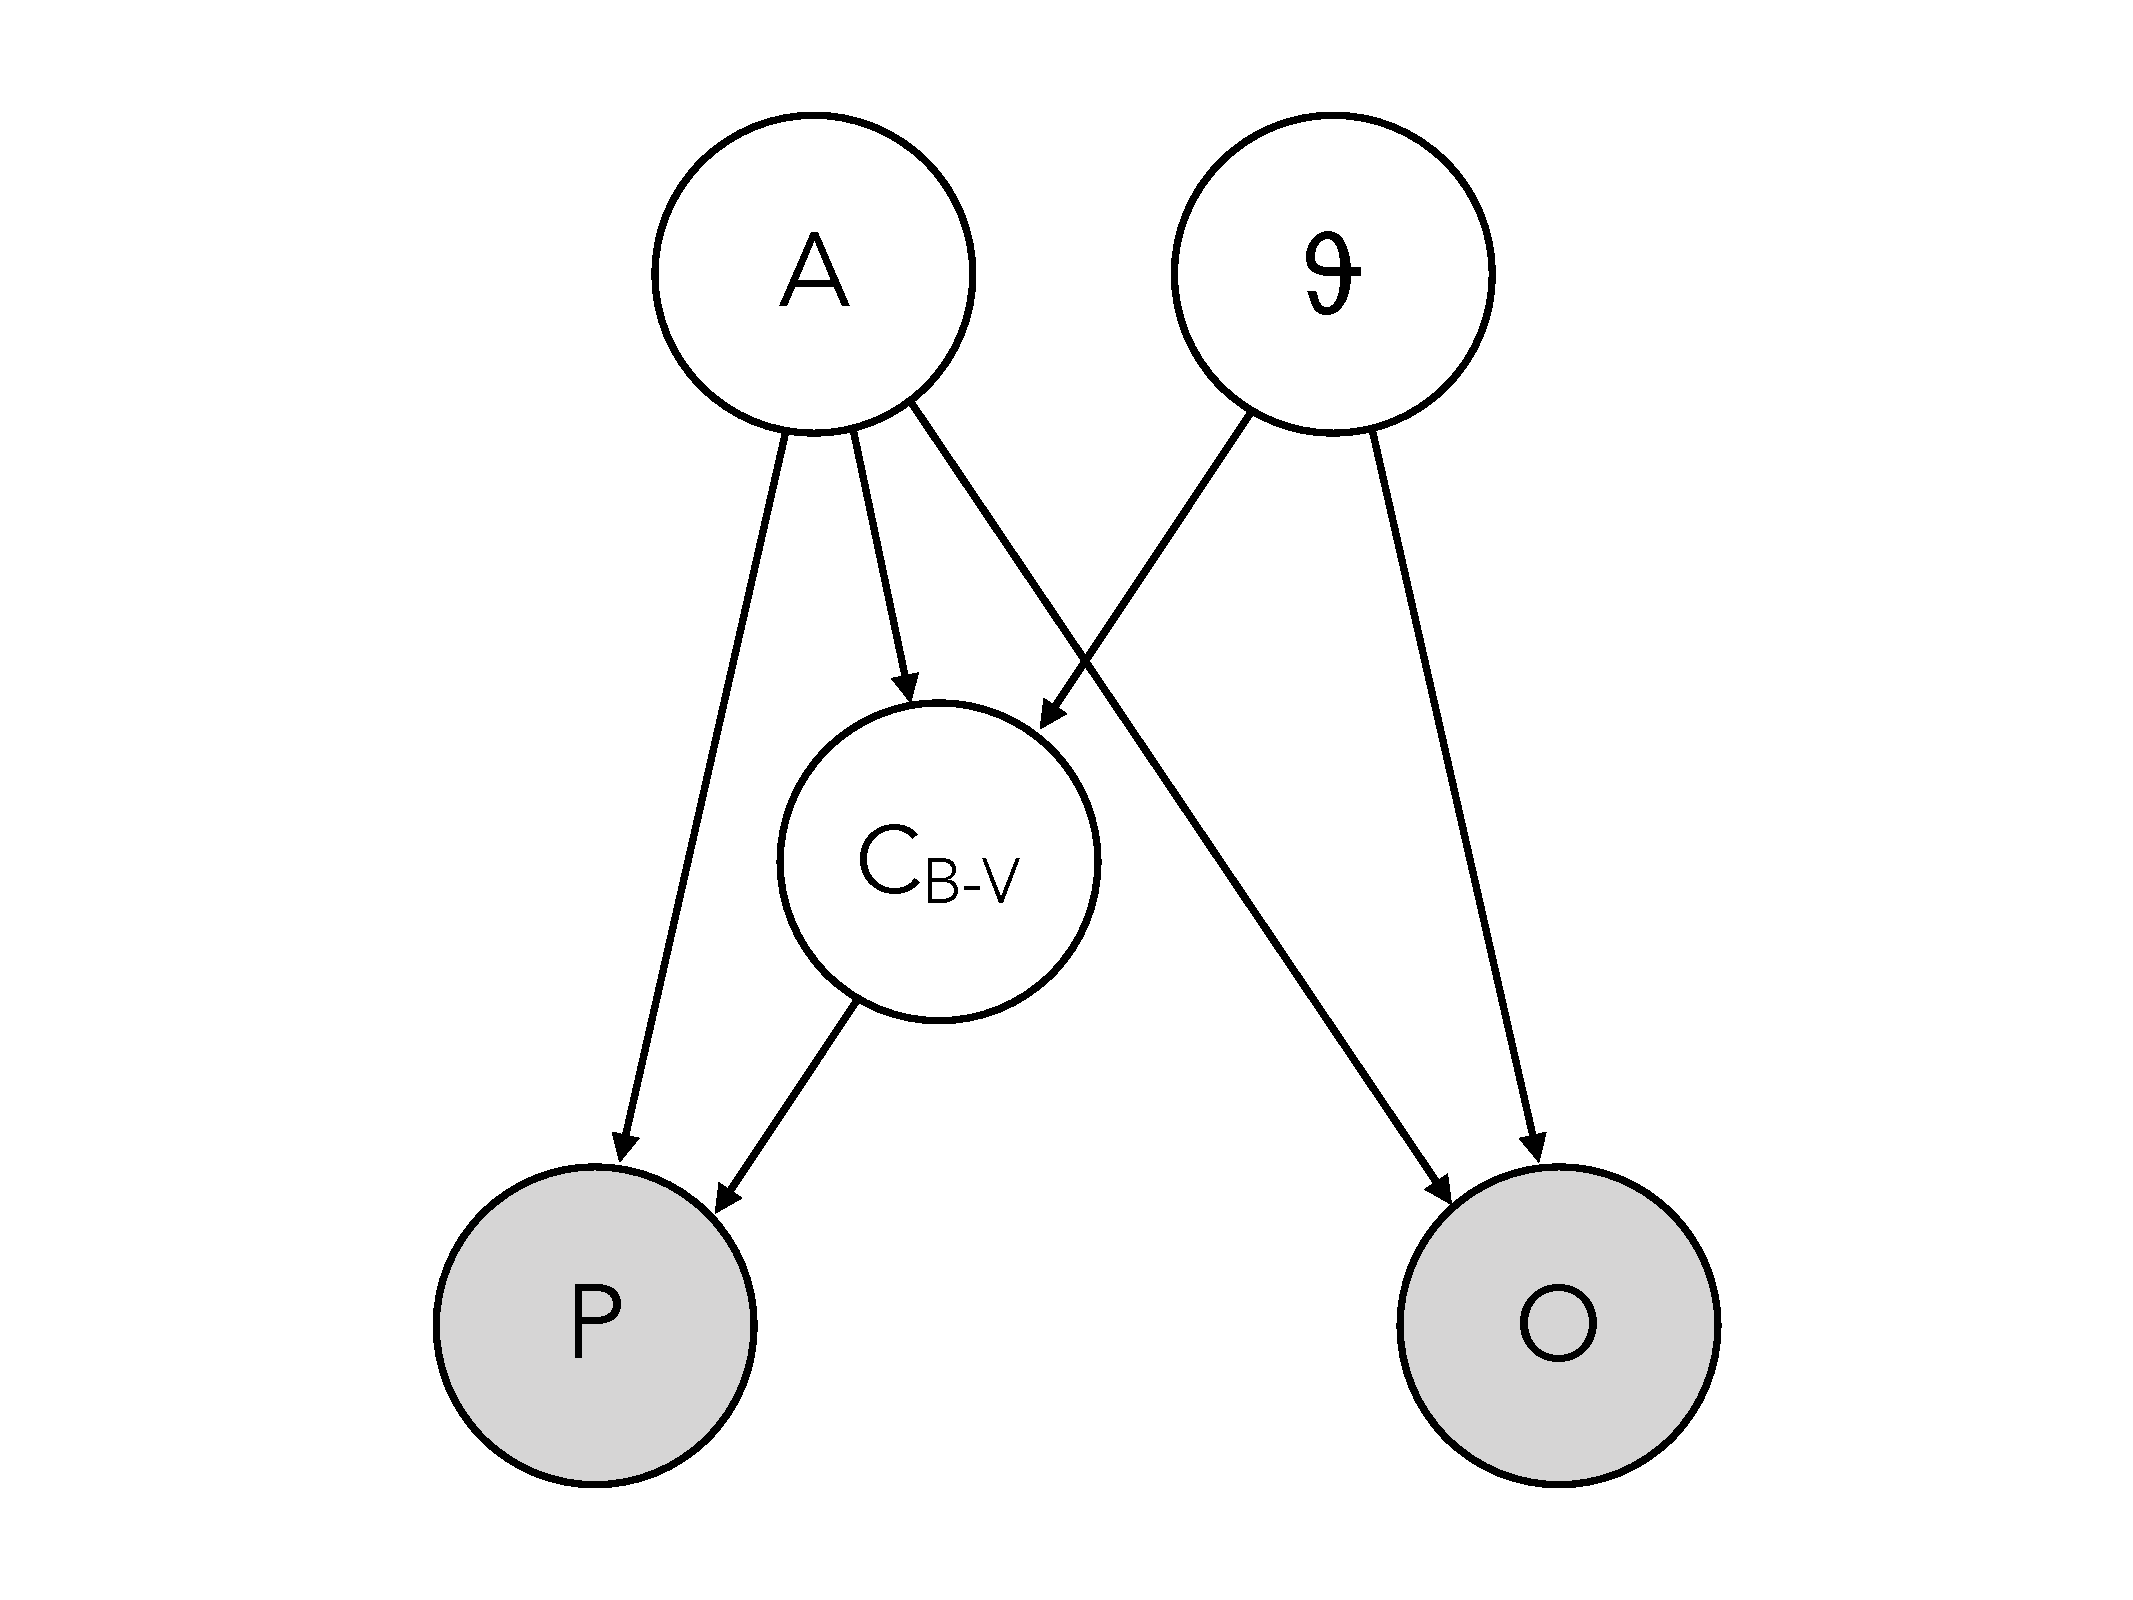
\includegraphics[width=.7\textwidth]{PGM}
\end{figure}
\label{fig:PGM}

%   - The formulas
The factorization of the likelihood described in equation \ref{eqn:factorized}
and depicted in figure \ref{fig:PGM} allows us to multiply two separate
likelihood functions together: one computed using an isochronal model and one
computed using a gyrochronal model.
The isochronal likelihood function is,
\begin{equation}
\mathcal{L} = p({\bf m_x}, T_{\mathrm{eff}}, \log g, \hat{F}, \bar{\omega}, B-V|A, M, D,
    A_V, F) \nonumber
\end{equation}
\begin{equation}
    = \frac{1}{\sqrt{(2\pi)^n \det(\sum)}}
    \exp\left( -\frac{1}{2} ({\bf O_I} - {\bf I})^T \sum ^{-1}
    ({\bf O_I} - {\bf I})\right),
\end{equation}
\label{fig:iso_likelihood}
where ${\bf O_I}$ is the vector of $n$ observables: \teff, \logg, \fhat,
\pmega, \mj, \mh\ and \mk, ${\bf I}$ is the vector of corresponding
predictions, calculated using an isochrone model, and $\sum$ is the covariance
matrix of the set of observables.
We assume there is no covariance between these observables and so this
covariance matrix consists of individual parameter variances along the
diagonal with zeros everywhere else.
To calculate ${\bf I}$, the vector of predicted observables, we use the
{\tt isochrones.py} package.
A detailed description of the isochronal model is provided later in this
manuscript.
The gyrochronal likelihood function is,
\begin{equation}
\mathcal{L} = p(P_{\mathrm{rot}}|A, B-V) \nonumber
\end{equation}
\begin{equation}
    = \frac{1}{\sqrt{(2\pi) \det(\sum_P)}}
    \exp\left( -\frac{1}{2} ({\bf P_O} - {\bf P_P})^T \sum ^{-1}
    ({\bf P_O} - {\bf P_P})\right),
    % = \prod_i \frac{1}{\sqrt{2\pi}\sigma_i} \exp
    % \left(-\frac{(P_{\mathrm{obs}, i} - P_{\mathrm{pred},
    % i})^2}{2\sigma_i^2}\right),
\end{equation}
\label{eqn:gyro_likelihood}
% where $P_{\mathrm{obs}, i}$ is the $i$th observed rotation period,
% $P_{\mathrm{pred}, i}$ is the corresponding predicted rotation period,
% calculated from the $i$th age and B-V values predicted by the isochronal
% model.
where $P_O$ is a 1-D vector of observed rotation periods, $P_P$ is the vector
of corresponding predicted rotation periods, calculated using the $i$th age
and B-V values predicted by the isochronal model.
The full likelihood function used in our model is the product of these two
likelihood functions,
\begin{equation}
    \mathcal{L} = \frac{1}{\sqrt{(2\pi)^n \det(\sum)}}
    \exp\left( -\frac{1}{2} ({\bf O_I} - {\bf I})^T \sum ^{-1}
    ({\bf O_I} - {\bf I})\right) \nonumber
\end{equation}
\begin{equation}
    \times
    \frac{1}{\sqrt{(2\pi) \det(\sum_P)}}
    \exp\left( -\frac{1}{2} ({\bf P_O} - {\bf P_P})^T \sum ^{-1}
    ({\bf P_O} - {\bf P_P})\right),
\end{equation}

%   - A description and reiteration in words.
A common approach to age-dating a star is to make separate age predictions
using separate sets of observables.
For example, if the rotation period, parallax and apparent magnitudes in a
range of bandpasses were available, one could compute both the gyrochronal age
of a star and its isochronal age.
How these two age predictions are later combined is then a difficult choice.
Is it best to average these predictions or just use the more precise of the
two or the one believed to be more accurate?
The methodology described here provides an objective method for combining age
estimates.
There is, after all only one age for each star.
If the two or more dating methods do not agree on the same age then one or
models must be inaccurate.
% More words about the implications of this.

%   - A word about the gyrochronology model.
The gyrochronology model we use to predict $P_P$ is, % $P_{\mathrm{pred}, i}$ is,
\begin{equation}
    P = A^\eta \alpha (B-V - \delta)^\beta,
\end{equation}
\label{eqn:gyro}
where $\eta$, $\alpha$, $\beta$ and $\delta$ are taken from \citet{angus2015}.
Although this gyrochronology model does not provide a good fit to all the
available data, we reiterate that no single model {\it is} able to reproduce
all the data, and that there is utility in using an extremely simple
functional form.
Again, this is not meant as a calibration exercise: in this paper we are more
concerned with introducing a new framework which allows an improved
gyrochronology model to easily be swapped in for this one.

% Practicalities: sampling, etc.
%-----------------------------------------------------------------------------
%   - isochrones.py
{\tt isochrones.py} is a {\it python} package with a range of functionalities
pertaining to isochrone fitting.
The first of the {\tt isochrones.py} functions we use is the likelihood
function of equation \ref{eqn:iso_likelihood}.
The {\tt isochrones.py} likelihood function takes a dictionary of observables
which can but does not have to include all of the following: \teff, \logg,
\feh, parallax and apparent magnitudes in a range of colors, as well as the
uncertainties on all these observables.
It then calculates the residual vector $({\bf O_I} - ({\bf I})$ where ${\bf
I}$ is a vector of predicted observables.
The prediction is calculated using a set of isochrones (we use the MIST
isochrones) where the set of model observables that is closest to the set of
real observed values is returned.
This requires interpolation over the model grids since, especially at high
dimensions, it is unlikely that an isochrone model is computed at exactly the
\teff, \logg, \feh, etc of the data, especially when those observations are
noisy.
% How does the interpolation work?
% How is the distance calculated?
The valid observable parameters predicted by the isochrone model that {\it
most closely} match the observations within the uncertainties go into ${\bf
I}$ and the {\tt isochrones.py} likelihood function returns equation
\ref{eqn:iso_likelihood}.
The second {\tt isochrones.py} function we use is one that querys the best-fit
isochrone model chosen to predict ${\bf I}$ in order to predict the B-V color
of that model.
This color is then used to calculate the gyrochronal likelihood function of
equation \ref{eqn:gyro_likelihood}.

% Extinction

%   - Emcee
We sample the joint posterior PDF over age, mass, metallicity, distance and
extinction using the affine invariant ensemble sampler, {\tt emcee}
\citep{foreman-mackey2013}.

%   - Assessing convergence

%   - Median, or maximum likelihood?
